\documentclass[aps,prb,onecolumn,notitlepage,showpacs,floatfix,superscriptaddress]{revtex4-1}
\usepackage{dcolumn}
\usepackage{tabularx}
\usepackage{bm}
\usepackage{soul}
\usepackage{amsmath,amssymb,graphicx}
\usepackage[colorlinks=true,citecolor=blue,urlcolor=blue,linkcolor=blue]{hyperref}
\usepackage{environ}

\NewEnviron{eqnsplit}{%
\begin{equation}
\begin{split}
  \BODY
\end{split}
\end{equation}
}

\newcommand{\mrm}[1]{\mathrm{#1}}
\newcommand{\ang}{\mathrm{\AA}}

\bibliographystyle{apsrev4-1}

%%%%%%%%%%%%%%%%%%%%%%%%%%%%%%%%%%%%%%%%%%%%%%%%
\begin{document}

\title{Stoner Ferromagnetism}

\author{Avinash Rustagi}
\email{arustag@ncsu.edu}
\affiliation{Department of Physics, North Carolina State University, Raleigh, NC 27695}
%
\date{\today}
%%%%%%%%%%%%%%%%%%%%%%%%%%%%%%%%%%%%%%%%%%%%%%%%

\maketitle
%
In a non-magnetic system, we have equal number of spin up and spin down electrons ($n_{\uparrow}=n_{\downarrow}=n$). For Ferromagnetism to exist, there must be an imbalance. This is attributed to the presence of repulsive interaction.\\

Let us consider a simple model with on-site repulsion (i.e. an energy cost $U$ when two electrons occupy the same site). As per the Pauli exclusion principle, it is required that if two electrons were to occupy the same site, they need to have opposite spins. \\

With this in mind, let consider the situation when $\delta n$ down-spin spontaneously flip. Then the number of up spins $n_{\uparrow}= n + \delta n$ and the number of up spins $n_{\downarrow}= n- \delta n$. This restructuring of the spins leads to a change in the energy of the system. The potential energy of the system is given by $U_E = U n_{\uparrow} n_{\downarrow} $The change in potential energy is
\begin{equation}
dU_E = U(n+\delta n)(n-\delta n) - U n^2 = -U (\delta n)^2
\end{equation}
\begin{figure}[hbtp]
\centering
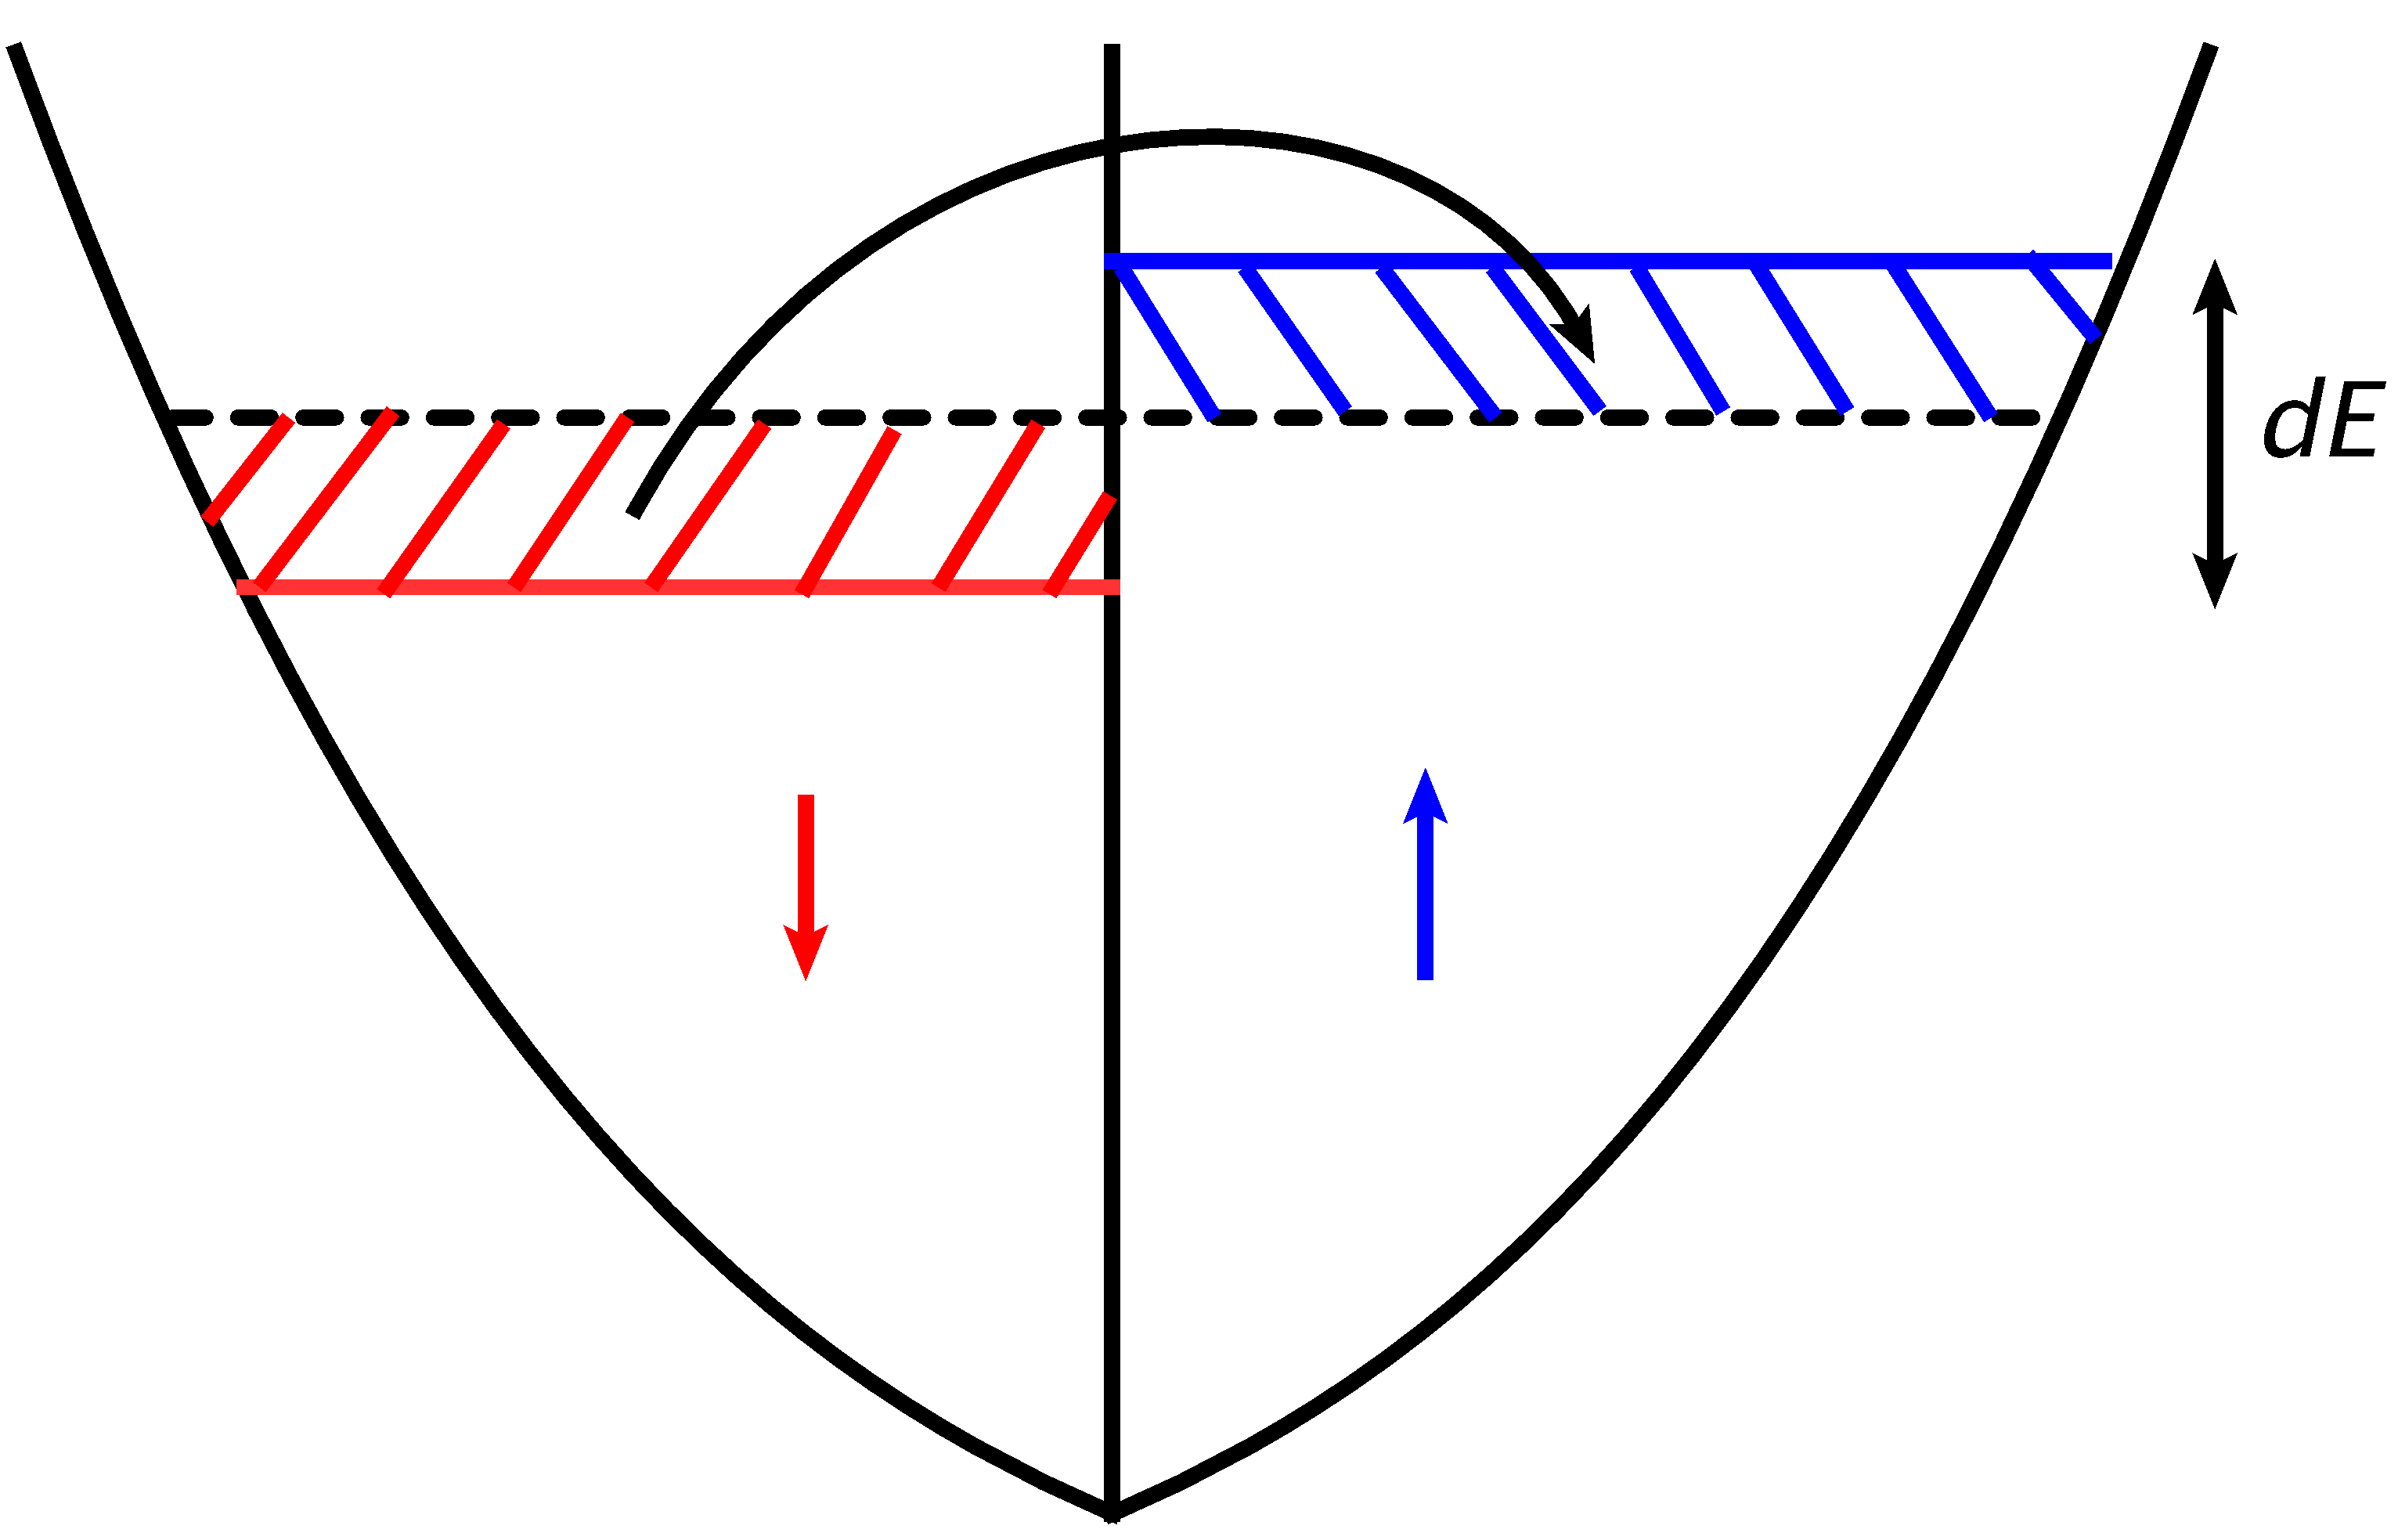
\includegraphics[scale=0.075]{Stoner.png}
\caption{Spontaneous change in the occupation of up/down spin states}
\end{figure}
The change in the kinetic energy due to the $\delta n$ spins occupying larger energy states is
\begin{equation}
dK_E= \delta n \, dE
\end{equation}
The density of states is defined as the number of states in the energy interval [$E,E+dE$]
\begin{equation}
D(E)=\dfrac{d n}{d E}
\end{equation}
Since the occupation change happens close to the Fermi level, we can relate the variation in number density $\delta n$ and the change in energy $dE$ through the density of states at the Fermi level.
\begin{equation}
\delta n =D_{F} dE 
\end{equation}
Thus the change in kinetic energy
\begin{equation}
dK_E = \dfrac{1}{D_F} (\delta n)^2
\end{equation}
The change in total energy is the addition of the kinetic and potential energy changes
\begin{eqnsplit}
dE_T &= dK_E+dU_E \\
&=\dfrac{(\delta n)^2}{D_F} \left[ 1-D_F U\right]
\end{eqnsplit}
The above equation provides the Stoner criterion for itinerant Ferromagnetism. When $D_F U /geq 1$, the system can lower its energy by creating an imbalance in the number of up and down spins, thereby becoming magnetic.
\end{document}